\chapter{Introduction}

..

\section{Introduction}

\subsection{On the output of Gpt unidirectional language models}
(TODO: intended meaning of the loss measure, sentence likelihood, contrast with sentence acceptability, .., ungrammatical sentences that are more likely than rarer grammatical ones, ..)
(math formulas of Gpt output, activation functions..)

C’è da aggiungere che la loss del modello gpt (score PenLP), usato come misura di accettabilità, è in realtà una stima globale della ..likelihood della frase (reference for this .. from gpt paper or other paper on ..transformers based language models). Ciò non corrisponde esattamente ad un giudizio di accettabilità/grammaticalità. Infatti, potrebbe darsi il caso, che una frase piuttosto comune (..) ma con un errore (sintattico, semantico, o altro) riceva una ..loss/likelihood maggiore di una frase. grammaticalmente corretta ma “rara”, o meglio, che usa un costrutto ricercato.. (es. ..).

\subsection{On the output of Bert-like bidirectional language models}
..

\subsection{Sentence acceptability estimates}

The Formula for the sentence acceptability estimates \( LP, PenLP \) from \citet{lau2020furiously} are:

\begin{displaymath}
	LP = \log P(s)
\end{displaymath}
\begin{displaymath}
	PenLP = \frac{LP}{((5+|s|) \big/ (5+1))^\alpha}
\end{displaymath}

Where \( P(s) \) is the probability of the sentence \( s \). The PenLP divides the \( LP \) estimate by a penalty term which depends on the sentence lenght \( |s| \), measured in number of tokens. Following \citet{lau2020furiously}, we use \( \alpha=0.8 \).

For Bert-like models, we use the estimate from \citet{lau2020furiously} of the log probability LP of a sentence s. It is estimated by masking each word in s, calculating the probability of the prediction of the masked word, and summing the log of all these probabilities:
..


\chapter{Experimental setup/design}
..

\subsection{Test description}
..

\subsection{Italian models details}

\textbf{Bert} (https://huggingface.co/dbmdz/bert-base-italian-xxl-cased): \textbf{81GB} (13 billion tokens) of training data  and from Wikipedia, OPUS and OSCAR corpora. Model 
 424 MB.

\textbf{GePpeTto} (LorenzoDeMattei/GePpeTto): \textbf{13.8GB} of training data from Wikipedia and ItWac corpus. The model’s size corresponds to GPT-2 small, with 12 layers and 117M parameters. Vocab size 30k. 620k training steps.

\textbf{GilBERTo} (https://huggingface.co/idb-ita/gilberto-uncased-from-camembert): Trained on \textbf{~71GB} of Italian text (11.2 billion tokens) from the OSCAR corpus. Model size 420 MB


\section{Factorial test design}
..



\subsection{Introduction}
..

Table with the four sentences of an example item ..

Four phenomena of island effect structures: whether, complex np, subject, and adjunct islands. Wh-dependencies (we leave rc-dependencies to future work.)
Two factors, dependency distance and presence or absence of an island structure. Each item has four sentences given by the combination of these two factors. We briefly call "short-nonisland" the sentence with a short-distance dependency and the lack of an island structure. For instance, for .. islands, we have these four ..

\renewcommand{\labelenumi}{(\arabic{enumi})}
\begin{enumerate}
	\item \textsc{Adjunct islands}
	\renewcommand{\labelenumii}{\alph{enumii}.}
	\begin{enumerate}
		\item \textsc{Short-NonIsland:} \\
		Chi dice che l’autore avrebbe inviato il libro all’editore?
		\item \textsc{Long-NonIsland:} \\
		Che cosa dici che l'autore avrebbe inviato all’editore?
		\item \textsc{Short-Island:} \\
		Chi ha stampato l’illustrazione dopo che l'autore ha inviato il libro all’editore?
		\item \textsc{Long-Island:} \\				
		Che cosa il disegnatore ha stampato l’illustrazione dopo che l'autore ha inviato all’editore?
		
	\end{enumerate}
\end{enumerate}

\subsubsection{Using factorial sentences as minimal pairs}
..
Using sentences from the factorial design to do minimal pairs comparisons and get accuracy scores ..)
..

\subsection{Test suites}

For the present thesis, we develop a new test suite that follows the same paradigm form as the one in \citet{sprouse2016experimental}, but with an increased item number of 50 (from the original 8). As in the original test suite in \citet{sprouse2016experimental}, there are four island phenomena (whether islands, complex np islands, subject islands, and adjunct islands). Each phenomena is exemplified in 50 items, which in turn are composed by four sentences covering the combinations of two factors: presence or absence of an island structure, and a short or long-distance dependency.

In the present work we treat only wh-dependencies and leave relative clause dependencies for future work.

Here is a sample item for whether islands:
..

Descritpion: ..

Here follows a sample item for the other 3 island structure types

\subsubsection{Scores normalization}

To be more directly comparable with the results in \citet{sprouse2016experimental}, the scores (LP or PenLP) were then discretized into a 7-point likert scale (using bins rather than quantiles) and normalized into z-scores.
The The likert scale discretization and the z-score normalization where done considering as an individual subject a model (like a Gpt-2 instance) paired with a particular sentence acceptability approximation (LP or PenLP), and taking all its scores across the four wh-dependency island effects phenomena of a particular test suite.

\chapter{Results}
..

\section{Accuracy results on island effects minimal pairs in Italian}
..

\subsection{Results table}

Results description: ..

The results are shown in \autoref{tab:accResults}.

\begin{table} \scriptsize 
	\begin{center}
		\begin{tabular}{p{0.095\linewidth}|p{0.099\linewidth}|c|p{0.04\linewidth}|c|p{0.04\linewidth}|p{0.04\linewidth}|p{0.04\linewidth}|c|p{0.04\linewidth}|c|p{0.04\linewidth}|}
			  &  & \multicolumn{2}{c|}{\textbf{Gpt2 (it)}} & \multicolumn{4}{c|}{\textbf{Bert (it)}}  & \multicolumn{4}{c|}{\textbf{GilBERTo (it)}} \\
			 \textbf{Pheno-menon} & \textbf{Sentence form} & LP & Pen LP & LP & Pen LP & LP-L & Pen LP-L & LP & Pen LP & LP-L & Pen LP-L \\
			\hline
			\multirow{3}{0.8cm}{Wh-adjunct}  & Short-N.I. & \textbf{96} & 92 & 94 & 90 & \textbf{96} & \textbf{96} & 86 & 70 & 86 & 86 \\ 
				%	\cline{2-12}
		  			   & Long-N.I. & \textbf{98} & 86 & 66 & 40 & 60 & 58 & 64 & 34 & 4 & 4 \\ 
		  		%	   \cline{2-12}
		  			   & Short-I.S. & 96 & 98 & \textbf{100} & 98 & \textbf{100} & \textbf{100} & 94 & 94 & 84 & 88 \\ 
		  	\hline
		  	\multirow{3}{0.8cm}{Wh-complex np} & Short-N.I. & 90 & 92 & \textbf{100} & \textbf{100} & 96 & 96 & 74 & 76 & 88 & 88 \\ 
		  			  		& Long-N.I. & \textbf{100} & 42 & 96 & 92 & 70 & 64 & 62 & 28 & 32 & 28 \\ 
		  					& Short-I.S. & 38 & 88 & \textbf{100} & \textbf{100} & 96 & 96 & 46 & 82 & 88 & 88 \\ 		  			 
		  	\hline
		  	\multirow{3}{0.8cm}{Wh-subject} & Short-N.I. & \textbf{98} & 90 & 26 & 6 & 28 & 28 & 70 & 46 & 28 & 22 \\ 
		  	& Long-N.I. & \textbf{100} & 98 & 86 & 56 & 78 & 74 & 76 & 50 & 24 & 20 \\ 
		  	& Short-I.S. & 40 & 56 & 62 & 60 & \textbf{68} & \textbf{68} & 52 & 56 & \textbf{68} & \textbf{68} \\ 
		  	\hline
		  	\multirow{3}{0.8cm}{Wh-whether} & Short-N.I. & 91.5 & 94.9 & 94 & 90 & \textbf{96} & \textbf{96} & 91.5 & 94.9 & 89.8 & 89.8 \\ 
		  	& Long-N.I. & \textbf{100} & \textbf{100} & 66 & 40 & 60 & 58 & \textbf{100} & 98.3 & 78 & 78 \\ 
		  	& Short-I.S. & 59.3 & 96.6 & \textbf{100} & 98 & \textbf{100} & \textbf{100} & 37.3 & 69.5 & 93.2 & 93 \\ 		  	
		\end{tabular}
		\caption{Accuracy results for Gpt-2 and Bert Italian models, on a test suite of 50 items per phenomenon. The Gpt2-it model is LorenzoDeMattei/GePpeTto. The Bert-it model is dbmdz/bert-base-italian-xxl-cased. The GilBERTo-it model (an Italian RoBERTa variant) is idb-ita/gilberto-uncased-from-camembert.}
		\label{tab:accResults}
	\end{center}
\end{table}

..
\subsection{Discussion}
..
Compare with accuracy scores on Blimp (English)
(also table with accuracy scores on Sprouse test suite)


\section{Factorial tests results}

% todo: regenerate Sprouse's plots from the published score data?

% Fig.1 Results from Sprouse et al (2016)
% Fig.2 Results of acceptability judgements to the same stimuli from Sprouse et al. 2016 from an Italian Gpt-2 model (GePpeTto) with the PenLP acceptability ..score. 
% Fig.3

\subsection{Differences between the plots}

In this section we discuss the results and plots with the Gpt-2 model and the PenLP sentence acceptability measure, since this combination seems to produce in general more accurate results. We include in the appendix the plots for the Bert models and the other acceptability measures (LP and PenLP based either on the model outputs after softmax of logistic activation functions).
% TODO: also model outputs based on a logistic function, but as a probability (divide for the sum of all the scores, but without the skewed exponential effect of the softmax)
..


\subsubsection{Complex np islands}

Here is a sample item from the complex NP island test suite we developed for this thesis:

\renewcommand{\labelenumi}{(\arabic{enumi})}
\begin{enumerate}
	\item \textsc{Complex NP islands}
	\renewcommand{\labelenumii}{\alph{enumii}.}
	\begin{enumerate}
		\item \textsc{Short-NonIsland:} \\
		Chi ha smentito che l'agenzia avrebbe diffuso il sondaggio? \\
		(`Who denied that the agency had released the poll?')
		\item \textsc{Long-NonIsland:} \\
		Cosa hai smentito che l'agenzia avrebbe diffuso? \\
		(`What have you denied that the agency had released?')
		\item \textsc{Short-Island:} \\
		Chi ha smentito la voce che l'agenzia avrebbe diffuso il sondaggio? \\
		(`Who denied the rumor that the agency had released the poll?')
		\item \textsc{Long-Island:} \\				
		Cosa hai smentito la voce che l'agenzia avrebbe diffuso? \\
		(`What have you denied the rumor that the agency had released?')
		
	\end{enumerate}
\end{enumerate}

In the middle and right images on \autoref{fig:wh_complex}, we see that, for complex NP items, the long non-island sentences on average get scored by the Gpt-2 model with a lower acceptability than by the human subjects (left image). This seems to be due to the long distance dependency effect, that gets exacerbated as a sentence increases in lenght (in these test suites, the complex NP islands examples have longer sentences).

\begin{figure}
	\centering
	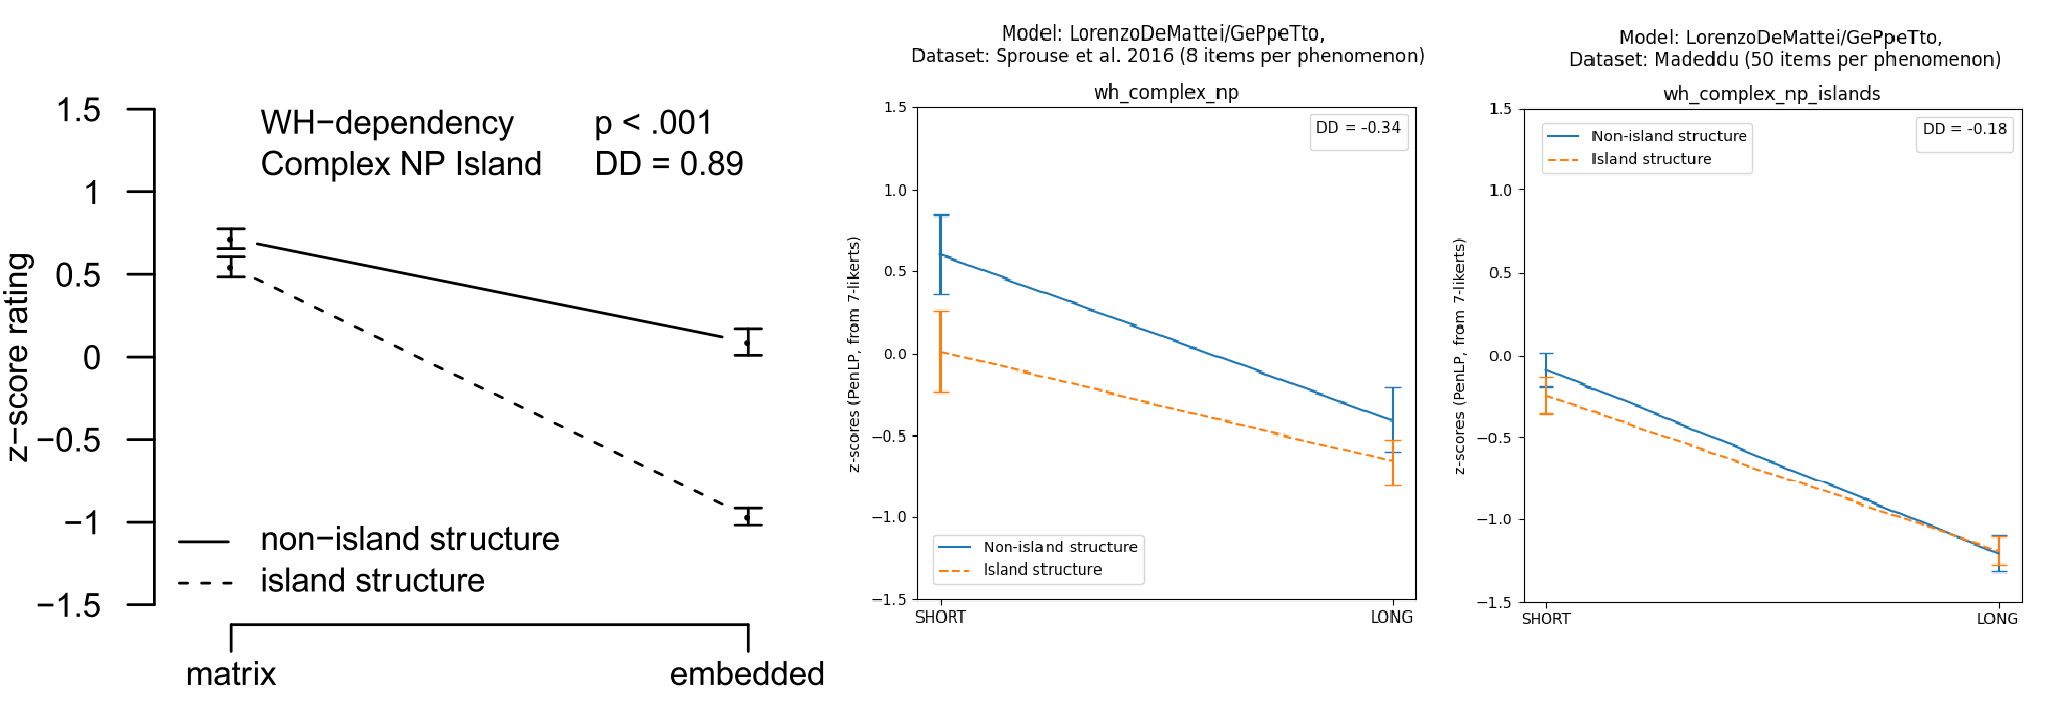
\includegraphics[width=1\textwidth]{images/Chapter1/combined_wh-complex.png} 
	\caption{Comparison of plots for wh-dependencies complex NP islands} 
	\label{fig:wh_complex} % this internally labels the figure for future referencing.
	\medskip
	\small
	The first plot on the left shows the scores on humans subjects published in \citet{sprouse2016experimental} for Italian complex NP islands with wh-dependencies. For each line, the left-most edge represents the score for the short-distance dependency sentence, the right-most the long-distance dependency. The plot in the middle shows the scores from a Gpt-2 model \citep{de2020geppetto} on the same test suite used for the first plot. The plot on the right shows the scores from the same Gpt-2 model but on the expanded test suite developed for the present thesis.
\end{figure}

Doing some variations experiments (see  \autoref{tab:compare1}), we found that by replacing the main clause verbs with "intuire che"/"avere l'intuizione che" ("to sense that" / "to have the intuition that") or "avvertire che"/"avere il sentore che" ("to feel that" / "to have an inkling that") or "percepire che"/"avere la percezione che" ("feel that"/"to have the feeling that"), the island restriction violation seem to have no effect, and the Long-Island sentence becomes more acceptable than the same sentence without the island structure (Long-NonIsland). \\ 
An hypothesis, whose demonstration we leave for future work, is that this is due to main clause expressions in which the subject has the semantic role of an \textsc{experiencer} rather than an \textsc{agent}, which could be a condition for Complex NP island restrictions to enter into effect or not. Indeed, the sentence \textit{Cosa hai avuto l'intuizione che il portavoce avrebbe confermato?} (\textit{`What did you have the intuition that the spokeperson had confirmed?'}), seems acceptable despite extracting from a complex NP construct.
% "avrebbe ppt" (condizionale passato)
% In fact, it seems that the Gpt-2 model correctly captures the fact that with these constructs the long nonisland sentences become acceptable.

\begin{table} \scriptsize 
	\begin{center}
		\begin{tabular}
			{p{0.3\linewidth} p{0.08\linewidth} p{0.3\linewidth} p{0.08\linewidth} p{0.08\linewidth}|} \\
			\multicolumn{2}{c}{\textbf{\textsc{Long-NonIsland}}} & \multicolumn{2}{c}{\textbf{\textsc{Long-Island}}}  &   \\
			\textbf{text} & \textbf{PenLP} & \textbf{text} & \textbf{PenLP} &  \textbf{Diff}  \\
			\hline
			\textit{Cosa hai messo in dubbio che il portavoce avrebbe confermato?} & -31.65
			& \textit{Cosa hai messo in dubbio la previsione che il portavoce avrebbe confermato} & -33.21 & 1.56 \\ 
			\textit{Cosa hai intuito che il portavoce avrebbe confermato?} & -32.36 
			& \textit{Cosa hai avuto l'intuizione che il portavoce avrebbe confermato?} & -29.99 & -2.37 \\ 	
			% TODO: use the other verbs too:  "avvertire che"/"avere il sentore che" ,  "percepire che"/"avere la percezione che" 
			\textit{Cosa hai detto che Gianni avrebbe sollevato?} & -33.74 
			& \textit{Cosa hai riferito il fatto che Gianni avrebbe sollevato?} & -36.64 & 2.90 \\ 
			\textit{Cosa hai intuito che Gianni avrebbe sollevato?} & -34.31 
			& \textit{Cosa hai avuto l'intuizione che Gianni avrebbe sollevato?} & -30.52  & -3.79 \\ 
			
			\textit{Cosa hai messo in dubbio che io avrei vinto?} & -26.48 & 
			\textit{Cosa hai messo in dubbio la previsione che io avrei vinto?} & -30.17 & 3.69\\ 				
			\textit{Cosa hai intuito che che io avrei vinto?} & -29.49 & 
			\textit{Cosa hai avuto l'intuizione che io avrei vinto?} & -24.45  & -5.04 \\ 				

		\end{tabular}
		\caption{Comparing acceptability variations among sentences in the complex NP dataset. A positive difference indicates that the Long-NonIsland sentence is more acceptable than the Long-NonIsland one, as expected.}
		\label{tab:compare1}
	\end{center}
\end{table}



With other variations experiments, we found that replacing the main clause verb with .."sapeva che"/"conosceva che" ("he knew that", see examples in table ..), increases the acceptability of the long-non island sentences; on the other hand, this variation results in a lower acceptability to the short island sentence, compared to the scores from human subjects, and by this way the non-island and island line end up being almost parallel, with the DD score is close to zero, indicating an almost absent island effect.
% todo: show tables with examples "sapeva che" % todo: numbered examples like formulas
% todo: show the plots for "intuizione che", "sapeva che" (two subfigures, each numbered/lettered to be referenced)

% examples of complex np items before and after the "avuto l'intuizione che" variation: ..
% show the plots for the items using this construct ("avuto l'intuizione che" ), it seems strange scores are given
% (the island line is higher than the non island one, but they are all acceptable sentence and there is no island restriction anymore)

% still the problem overall in the orginal plots seems an overly low score for the long non island sentences
% that is, is the long distance depencency that receives a too loo score .. (lenght effect?)
% while the structure effect ..
% albeit it's correct, like humans scores, that the long non island has less acceptability than the short island
% then how is the long distance dependency (lenght effect) scored for the other island phenomena?
% the difference with the sentences for the other phenomena seem to be that they have a simpler main clause, like "cosa pensi che" (present) + "abbia ppt"  (congiuntivo passato), while for the complex np, is "cosa hai smentito/annunciato/raccontato/sostenuto che" (passato prossimo) + "avrebbe ppt" (condizionale passato)
% a comparison example could be to turn the other 3 island phenomena items into passato prossimo for the main clause
% but was this discrepancy also in Sprouse data, and is this the reason for their plots differences too? (so the gpt2 model just accentuates this drop in acceptability?)

% for future work: automatic generation of examples from templates, like in Blimp, to control and test more easily for more factors (es. verbs modes and tenses)
% to test for frequency effect: use some rare verb modes/tenses?

% also find an explanation for the other misclassified long non island sentences that use other constructus (with proper agent/patient semantic roles)

% table..

% Mostra una non robustezza del modello nell’apprendimento di strutture sintattiche / or of this use for scoring minimal pairs, non generalizzazione sintattica, in quanto basta una variazione lessicale, anche tra ..parole frequenti, ..per ..alterare ..quale tra due frasi coppie minime sia piu o meno accettabile.
% However, we refer back to section .., about the interpretation/meaning of the Gpt-2 loss ..output/score.


% TODO: table with example items with different constructs, and their scores
% TODO: plots of the whole test suite for this phenomenon with the same variation for all items (using a different verb)



\subsubsection{Whether islands}

From \autoref{fig:wh_whether} for whether islands with wh-dependencies, we can see that the Gtp-2 model, with the PenLP sentence acceptability estimate, compared with the results from humans gives higher scores for all sentence types. This difference is more pronounced in the scores on the original test suite from \citet{sprouse2016experimental} (middle image). The slope of the lines (both for island and non-island sentence structures) is however quite similar to the human scores. \\
The Gpt-2 scores on the original Sprouse et al. test suite (middle image) have wider standard error bars, which are considerably smaller for the new test suite developed for the present thesis (right image).\footnote{This might be due to the fact that the number of items between the two test suites increases from 8 to 50.}

\begin{figure}
	\centering
	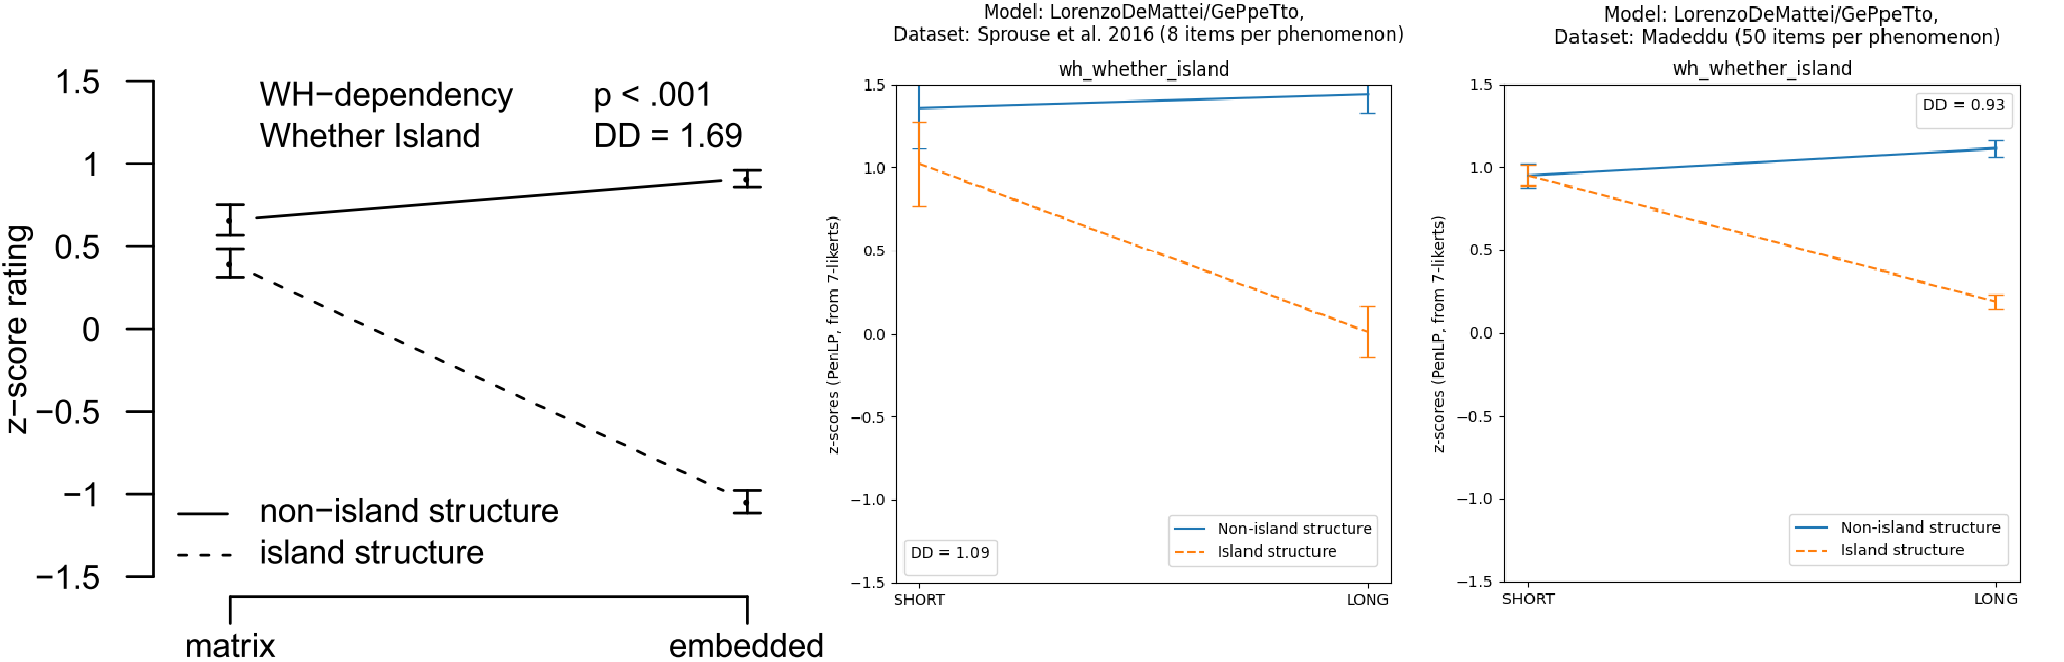
\includegraphics[width=1\textwidth]{images/Chapter1/combined_wh-whether.png} % width= 0.8\textwidth
	\caption{Comparison of wh-dependency whether islands} 
	\label{fig:wh_whether} % this internally labels the figure for future referencing.
\end{figure}

..
\renewcommand{\labelenumi}{(\arabic{enumi})}
\begin{enumerate}
	\item \textsc{Whether islands}
	\renewcommand{\labelenumii}{\alph{enumii}.}
	\begin{enumerate}
		\item \textsc{Short-NonIsland:} \\
				Chi pensa che io abbia riscosso il pagamento?
		\item \textsc{Long-NonIsland:} \\
				Cosa pensi che io abbia riscosso?
		\item \textsc{Short-Island:} \\
				Chi si domanda se io abbia riscosso il pagamento?
		\item \textsc{Long-Island:} \\				
				Cosa ti domandi se io abbia riscosso?
				
	\end{enumerate}
\end{enumerate}

% TODO: table showing accuracy scores for the 4 sentences of an item; comparison on variations across multiple items


\subsubsection{Subject islands}

\begin{figure}
	\centering
	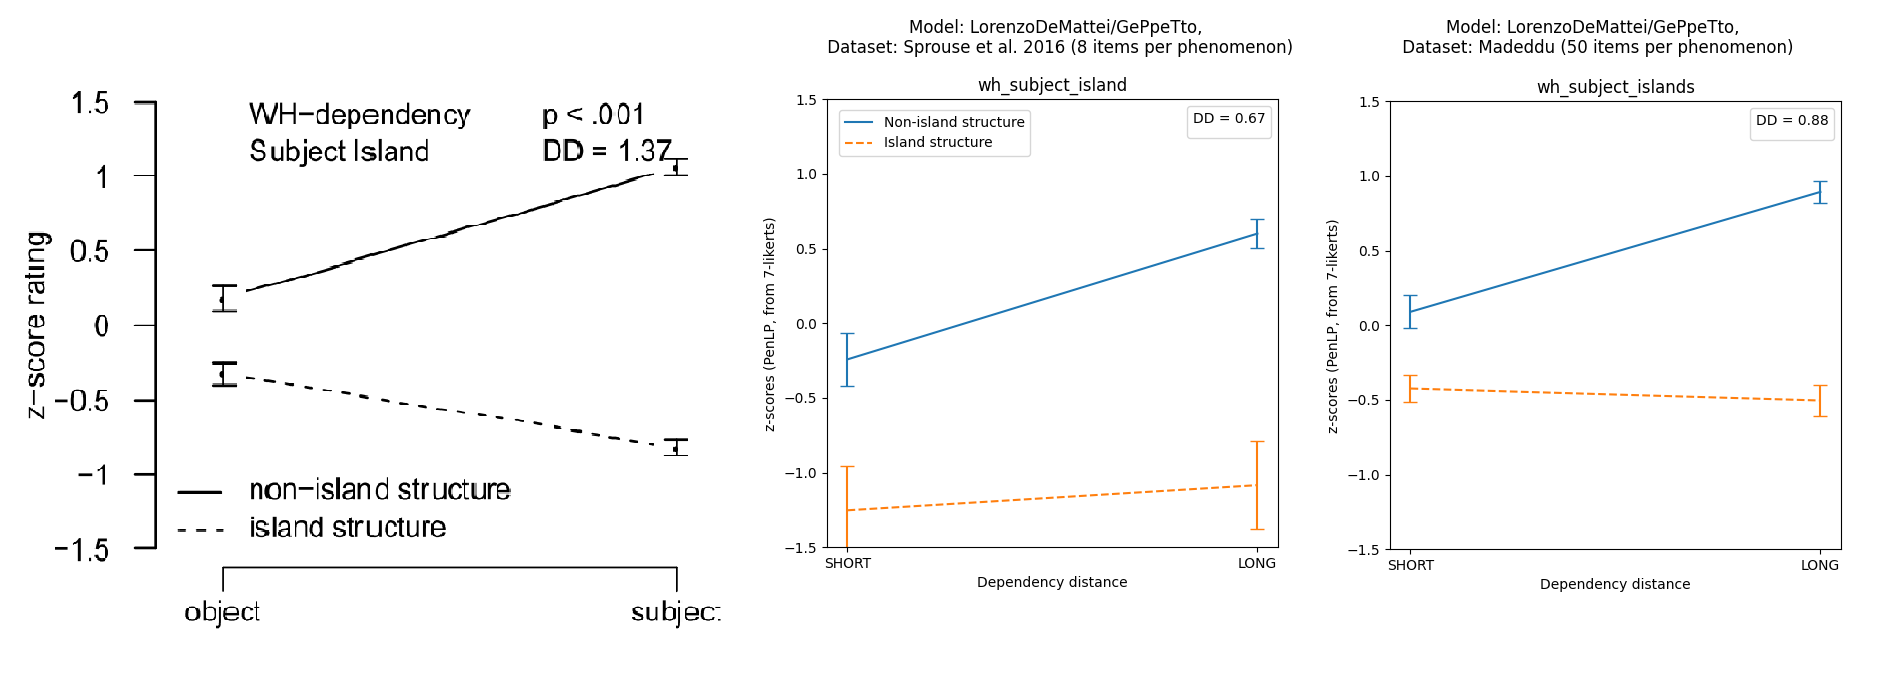
\includegraphics[width=1\textwidth]{images/Chapter1/combined_wh-subject.png} 
	\caption{Comparison of wh-dependencies subject islands} 
	\label{fig:wh_subject} % this internally labels the figure for future referencing.
\end{figure}

In \autoref{fig:wh_subject}

on Sprouse data, island line is significantly lower (check sorting of sentences to see why). On new data, is similar. \\
For the non island line, the short point is lower on both sprouse and new data. \\ 
The long point is similar on new data (around 1.0) but lower on sprouse data. \\
..The slope is similar on the model scores, both for sprouse and new data, but steeper compared to acceptability results on human subjects.


\subsubsection{Adjunct islands}

\begin{figure}
	\centering
	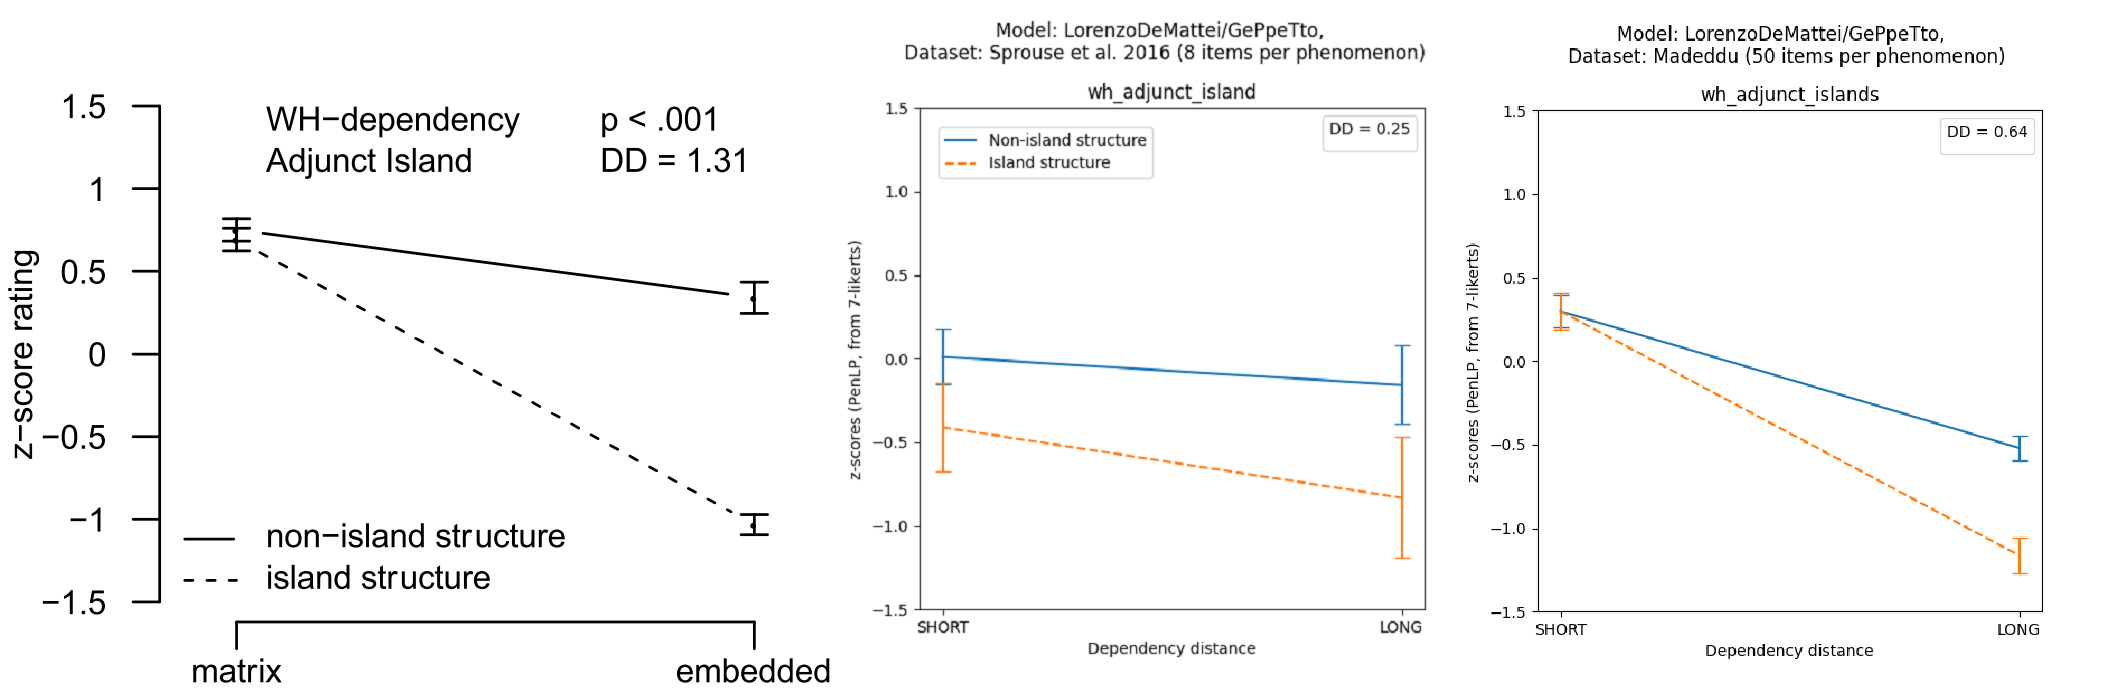
\includegraphics[width=1\textwidth]{images/Chapter1/combined_wh-adjunct.png} 
	\caption{Comparison of wh-dependencies adjunct islands} 
	\label{fig:wh_adjunct} % this internally labels the figure for future referencing.
\end{figure}


In \autoref{fig:wh_adjunct}

the non island line on new data is similar, althoughg with an higer acceptability for short non island, which results in a downward steeper line. The non island line is also similar on new data, albeight also with a steeper downward slope.
NB: the new data, for the long islands, has a more clearly unacceptable ..form: in the sprouse data, at the end there is a preprositional ..phrase like “in ufficio”.

\subsubsection{Overall}
..
While on human ratings the unacceptable sentences (long nonislands) receive all on average a z-score of about -1, there is more variability in the scores given by the models, in particular for whether islands sentences, which receive much higher acceptability rating on average.
..

% TODO: remaining tables with accuracy scores, comparison with Blimp extraction islands scores; compare btw models, scoring measures, and datasets (Blimp, Sprouse, Madeddu)

% todo: all the plots in the appendix (Bert, LP/PenLP, logistic LP/PenLP, .. ) and brief comments 
% (like limitations of Bert acceptability estimates)

% Italian models:
% "LorenzoDeMattei/GePpeTto"
% "dbmdz/bert-base-italian-xxl-cased": ModelTypes.BERT,
% "idb-ita/gilberto-uncased-from-camembert"

% testsuites/datasources:
% Sprouse et al.
% Madeddu

% scoring measures:
% LP/PenLP (softmax-based)
% % LP/PenLP (logistic-based)


\subsection{What seems to affect the models acceptability scores}
..

\subsubsection{Whether islands}
Replacing personal pronouns with proper nouns or .. (like “il parlamentare”, “lo studente”, ..) aligns more the scores with those of humans.
This might be the reason for the discrepancies in some of the 4 phenomena: some make more use of ..nomen agentis, while others rely more on personal pronuns.
Try this replacement this in all 4 test sets.

Not much difference seems to derive by using less common (..) verbs .. 
(examples in which both sentences in a pair also specify the direct object, see how this affects the score? Like long nonisland vs long island ..)


\subsubsection{Subject islands}
..

\subsubsection{Adjunct islands}

Guardando le short-nonislands, sembra anche qui preponderante il fatto di usare nomi propri di persona (che ha uno score di accettabilità minore) e usare invece di nomi comuni animati/di mestieri/.. (che aumenta l’accettabilità). Ma questo non sembra influenzare il DD score finale (..evidentemente i vari fattori si bilanciano).


\subsection{Discarded observations on differences between the plots}

\subsubsection{Other notes on  Complex np islands,  what seems to affect the models acceptability scores}
In \autoref{fig:wh_complex} we see that the non-island line (the line connecting the two acceptability scores for short and long distance dependency sentences without an island structure) is significantly lower in new data (todo: see constructs that increase the score of both long and short)

The (gpt) model seem not to make much difference in ..acceptability btw “regular” subordinates and complex noun phrases ..

-- also the short island point is significantly lower

All the 50 + 8 items of the two test suites (the ones from Sprouse et al and the ones developed for the present thesis), when altered to use the following construct for the complex NP "avuto l'intuizione che" (had the intuition that), are scored by the model as if there is no island restriction violation anymore. 

il verbo “intuire” diminuisce ..l’accuratezza del giudizio di accettabilità
in particolare diminuzione della accettabilità delle frasi long nonisland (con long distance wh dependency e struttura non island), che ricevono accettabilità minore di quelle con struttura island:
Esempio analisi variazioni con verbo “intuire” complex np, ..

the verb form “sapeva” (imperfect), compared to ..present perfect forms (“ha osservato/affermato/..”) seems to get better DD score in complex np islands (and also in another phenomenon ..).

\subsubsection{Whether islands}
NB: note that according to human scores, for this type of whether island sentences, the "correct" scoring is to have an increase in acceptability going from short to long non island sentences.
Maybe comparing the scores between acceptable sentences (in this case short and long non islands), expecting it to match humans acceptability judgements .. is beside the present ..research question.
In any case, we noted a reverse in the acceptability difference between this two types of sentences (short and long non islands) when changing the subject of the subordinate sentence from a personal pronoun ("io", 1st pers sg), to a proper noun (i.e. "Gianni"), to a common noun (i.e. "il parlamentare").

-- significant variation in acceptability diff between short non island and long non island, when replacing: the personal pronouns io/lei, with a proper noun like "Gianni", or even more with a noun like "il parlamentare" (the congressman). In this latter case, significant improvement toward the expected acceptability rate (only 10 out of 50 are .."missclassified"). With the proper noun "Gianni", 18 are missclassified. With the personal pronoun 29 out of 50 are missclassified.
Try replacing with .. another proper noun, more common like ..


(tables and examples of these variations to put on the thesis/report?)

(possible explanation: personal pronouns and proper nouns might be less common in the type/genre of corpora these models were trained on, like wikipedia).
Observations: the direct objects in the examples are all relatively common words..\footnote{\citet{wei2021frequency} found significant frequency effects (but for agreement .. tests, which are much easier to isolate), for items that occurr rarely in the training corpus (..less then ..10-100 times). But to notice this effect they had to purposly tweak the training corpus. Replicating this for a preexisting corpus (using very rare vocabulary ..) is much more complex and out of the scope of the present study.}
try with rarer ones.
..
-- both on sprouse and new data, gpt "incorrectly" increases the accceptability from short to long non island (check constructs that instead decrease the acceptability?)

\subsection{Future work}
..
Analizzare le attivazioni nei vari livelli del modello ..
Fare un training .”a strati”, in cui in ciascuno strato c’è il target dell’apprendimento di un livello di base della lingua (morfologia, sintassi, semantica, ampiezza del vocabolario, ..), con strati successivi che aumentano la complessità della conoscenza che il modello ha del linguaggio.


Confronto percentuali accuratezza (short/long non island, short island) con quelle in Blimp
(and other works with extraction islands evaluations?)


\section{Blimp English dataset}
..
\subsection{English models details}
..

\section{Misc notes with refs}

“NATURAL LANGUAGE DOES NOT MAXIMIZE PROBABILITY” 
“Why is human-written text not the most probable text? We conjecture that this is an intrinsic property of human language. Language models that assign probabilities one word at a time without a global model of the text will have trouble capturing this effect. Grice’s Maxims of Communication (Grice, 1975) show that people optimize against stating the obvious. Thus, making every word as predictable as possible will be disfavored. This makes solving the problem simply by training larger models or improving neural architectures using standard per-word learning objectives unlikely: such models are forced to favor the lowest common denominator, rather than informative language.” 
\citep{holtzman2019curious}

Repeated exposure to a type of island construct will increase its perceived acceptability 
\citep{chaves2014subject}

Targed ..syntactic tests on modern language models seem to have started with \citet{linzen2016assessing}, while the use of psycholinguistic tests for this seem to have started with \citet{futrell2018rnns}.

\clearpage
\section{More latex examples}
\subsection{..}
\subsubsection{This is a sub-subsection}
\section*{This is another section, but it gets omitted in the table of contents}
..


Listing bibliography entries \citep{wei2021frequency, hu2020systematic, lau2020furiously, sprouse2016experimental, bostrom2020byte, futrell-etal-2019-neural}

\subsubsection{This is another subsection}

What follows is an example of programming code. You can change the programming language and the corresponding syntax highlighinh scheme, adding keywords... For more info see the package guide \texttt{listings}.

\lstinputlisting[language=C++]{listings/Capitolo1/code1.cpp} 
